\documentclass{article}
\usepackage[utf8]{inputenc}
\usepackage[portuguese]{babel}
\usepackage{graphicx} % Required for inserting images
\usepackage{url,psfrag}
\usepackage{csquotes}
\usepackage{amsmath}
\usepackage{amsfonts}
\usepackage[
maxbibnames=99,
backend=bibtex,
%style=alphabetic,
sorting=ynt
]{biblatex} %Imports biblatex package
\addbibresource{bibliografia.bib}

\title{Algoritmo de Balas aplicado ao TSP com janelas de tempo e carro elétrico}

\begin{document}

\maketitle

%\section*{Identificação}

\noindent{\bf Orientador}:  Álvaro Junio Pereira Franco - \url{alvaro.junio@ufsc.br}\\

\noindent{\bf Estudante}: Felipe Lourenço da Silva - \url{felipe.lourenco@grad.ufsc.br}\\

\noindent{\bf Departamento}: Informática e Estatística\\

\noindent{\bf Centro de ensino:} Tecnológico\\

\noindent{\bf Título do projeto:} Modelos e algoritmos para variações modernas do problema de roteamento de veículos\\

\noindent{\bf Fonte financiadora:} Conselho Nacional de Desenvolvimento Científico e Tecnológico - Termo de Outorga - Processo: 405247/2023-0 (SIGPEX N. 202104940)

\section*{Resumo}
Adaptamos o algoritmo de Balas que resolve o TSP com janelas de tempo para resolver o TSP com janelas de tempo e carro elétrico.

\section*{O algoritmo de Balas}
O algoritmo de Balas foi apresentado no artigo \cite{Ba}. Uma implementação deste algoritmo foi apresentada em \cite{BS}. Vamos usar a mesma notação que aparece nos artigos citados. O grafo de entrada possui $n$ vértices e é completo. As $n$ cidades são indexadas por índices em $N=\{1, 2, \dots, n\}$. Muitas vezes escrevemos $i$ como o índice da cidade $i$. Uma permutação $\pi$ de $1, 2, \dots, n$ é uma solução do TSP clássico. A posição da cidade $i$ em uma solução viável do problema é denotado por $\pi(i)$. O grafo possui custos nas arestas $t_{ij}$ que representam tanto a distância quanto o tempo entre os vértices $i$ e $j$. O algoritmo de Balas resolve o TSP com a seguinte restrição: dado um inteiro positivo $k$ e qualquer par de cidades $i$ e $j$, se $j \geq i + k$ então em qualquer solução viável do problema, a cidade $i$ deve preceder a cidade $j$, ou seja, $\pi(i) < \pi(j)$. A este problema, vamos nos referir como TSP restrito. O algoritmo consiste de uma redução do TSP restrito para o problema de encontrar um caminho de menor custo em um grafo dirigido acíclico.

Existem condições necessárias importantes (mas não suficientes) que valem destacar. A primeira delas determina as cidades candidatas a ocupar uma determinada posição em uma solução viável, $\pi^{-1}$. As cidades candidatas a ocupar a posição $i$ de uma solução viável são aquelas dentro do intervalo de inteiros $\{\max\{1, i - k + 1\}, \dots, \min\{i + k - 1, n\}\}$. Podemos então escrever que uma cidade candidata $\pi^{-1}(i)$ atende a seguinte restrição $$\max\{1, i-k+1\} \leq \pi^{-1}(i) \leq \min\{i+k-1,n\}.$$ Para qualquer cidade $j$, a posição de $j$ em uma solução viável também está definida dentro do seguinte intervalo de inteiros $\{\max\{1, j-k+1\}, \dots \min\{j + k -1,n\}\}$, ou seja, $$\max\{1, j-k+1\} \leq \pi(j) \leq \min\{j+k-1,n\}.$$ Portanto, dada a ($i-1$)-ésima visita do caixeiro viajante a algum vértice do grafo, o próximo vértice $j$ a ser visitado poderá ser obtido através da construção de um grafo auxiliar considerando todas as possibilidades de vértices candidatos para a posição $i$ (ou seja, $\pi^{-1}(i) = \max\{1, i-k+1\}, \dots, \min\{i+k-1,n\}$) e considerando todas as posições que uma cidade $j$ pode ocupar (ou seja, $\pi(j) = \max\{1, j-k+1\}, \dots, \min\{j+k-1,n\}$). Caso alguma cidade candidata $j$ para a posição $i$ não esteja dentro do intervalo descrito acima, então essa cidade não deve ser considerada. Além disso, devemos ainda verificar a condição do TSP restrito: se $j \geq i + k$ então $\pi(i) < \pi(j)$.

O grafo auxiliar $G^*$ é construído com $n+1$ camadas. O conjunto de vértices da camada $i$ do grafo auxiliar é denotado por $V^*_i$. $V^*_1 = \{s\}$ (vértice fonte $s$). $V^*_{n+1} = \{t=s\}$ (vértice sorvedouro $t$ que é igual a fonte $s$). O número de vértices de uma cada $V^i_i$ é no máximo $(k+1)2^{k-2}$ para $i=2, \dots, n$. O grau de entrada de cada vértice do grafo auxiliar é no máximo $k$.

Em geral, a segunte recorrência calcula o custo de um segmento ótimo começando na cidade 1, passando pelas cidades de um subconjunto $W\subset N$ nas posições $2, \dots, i-1$ e visitando a cidade $j$ na posição $i$: $$C(W,i,j) = \min_{l\in W}\{W \backslash \{l\}, i-1, l\}.$$

No TSP clássico, existem muitas possibilidades para um conjunto $W$ com $i-2$ elementos, a saber, $\binom {n}{i-2}$. No entanto, no TSP restrito, as possibilidades para $W$ são poucas e descritas por pares de subconjuntos cujo tamanho de cada um é limitado por $k$. Os pares são:
$$ S^-(\pi, i):= \{l \in (1, \dots, n): l \geq i, \pi(l) \leq i-1\} \textmd{ e }$$
$$ S^+(\pi, i):= \{h \in (1, \dots, n): h \leq i-1, \pi(h) \geq i\}.$$

Descrevendo os conjuntos acima de outra forma, $S^-(\pi, i)$ é o conjunto de cidades de uma solução viável $\pi$ que possuem índices maiores ou iguais a $i$ e que foram visitadas em alguma posição $1, \dots, i-1$, enquanto que $S^+(\pi,i)$ é o conjunto de cidades de uma solução viável $\pi$ que possuem índices menores ou iguais a $i-1$ e serão visitadas em alguma posição $i, \dots, n$. É demonstrado que $|S^-(\pi, i)| = |S^+(\pi, i)| \leq \lfloor k/2 \rfloor$.

Um caminho de custo mínimo no grafo auxiliar passará por um vértice em cada camada do grafo. Um vértice deste caminho na camada $i$ contém a cidade que é visitada na posição $i$ da solução ótima. Um vértice na camada $i$ do grafo auxiliar é denotado por $(i, j, S^-_{ij}, S^+_{ij})$ sendo $j$ uma cidade candidata à posição $i$, e $S^-_{ij}$ e $S^+_{ij}$ sendo, respectivamente, $S^-(\pi, i)$ e $S^+(\pi, i)$. A construção dos vértices  $(i, j, S^-_{ij}, S^+_{ij})$ da camada $V^*_i$ é realizada considerando todos os candidatos $j$ para a posição $i$. Dessa forma, é possível obter todos os vértices da camada $V^*_i$. Os arcos de $G^*$ conectam vértices de camadas consecutivas. Dois vértices, $(i-1, l, S^-_{i-1, l}, S^+_{i-1, l})$ e $(i, j, S^-_{ij}, S^+_{ij})$ são adjacentes (\emph{compatíveis}) se cada caminho $T_{i,j}$ em $G$ que vai da cidade 1 até a cidade $j$ na posição $i$ pode ser obtido por um caminho $T_{i-1,l}$ em $G$ que vai da cidade 1 até a cidade $l$ na posição $i-1$. Ou seja, basta adicionar $j$ ao caminho $T_{i-1,l}$ para obter $T_{i,j}$. Os vértices de um caminho $T_{i,j}$ estão no conjunto $N(i,j,S^-_{ij}, S^+_{ij}) = (N_{i-1} \setminus S^+_{ij}) \cup S^-_{i,j}$. $N_i$ é uma notação para o conjunto das cidades $\{1, 2, \dots, i\}$. Com isso, vértices $(i-1, l, S^-, S^+)$ e $(i, j, S^-, S^+)$ são compatíveis se e somente se $$N(i, j, S^-_{ij}, S^+_{ij}) = N(i-1, l, S^-_{i-1,l}, S^+_{i-1,l}) \cup \{l\}.$$ Para obter os arcos de maneira eficiente, a última equação é expressa em termos dos conjuntos $S^-_{ij}$, $S^+_{ij}$, $S^-_{i-1, l}$ e $S^+_{i-1, l}$.

\paragraph{Proposição de Balas.} Os vértices $(i-1, l, S^-_{i-1, l}, S^+_{i-1, l})$ e $(i, j, S^-_{ij}, S^+_{ij})$ são adjacentes (compatíveis) se e somente se $j \neq l$ e vale uma das seguintes condições.
\begin{itemize}
\item Se $l < i-1$ e $i-1 \in S^-_{i-1, l}$, \\então $S^-_{ij} = S^-_{i-1,l}\setminus\{i-1\}$ e $S^+_{ij} = S^+_{i-1,l} \setminus \{l\}$.
\item Se $l < i-1$ e $i-1 \notin S^-_{i-1, l}$, \\então $S^-_{ij} = S^-_{i-1,l}$ e $S^+_{ij} = S^+_{i-1,l} \setminus \{l\} \cup \{i-1\}$.
\item Se $l = i-1$, \\então $S^-_{ij} = S^-_{i-1,l}$ e $S^+_{ij} = S^+_{i-1,l}$.
\item Se $l > i-1$ e $i-1 \in S^-_{i-1, l}$, \\então $S^-_{ij} = S^-_{i-1,l}\setminus\{i-1\} \cup \{l\}$ e $S^+_{ij} = S^+_{i-1,l}$.
\item Se $l > i-1$ e $i-1 \notin S^-_{i-1, l}$, \\então $S^-_{ij} = S^-_{i-1,l} \cup \{l\}$ e $S^+_{ij} = S^+_{i-1,l} \cup \{i-1\}$.
  
\end{itemize}

Para finalizar, o custo de um arco entre os vértices $(i-1, l, S^-_{i-1, l}, S^+_{i-1, l})$ e $(i, j, S^-_{ij}, S^+_{ij})$ em $G^*$ é o custo do arco entre os vértices $l$ e $j$ de $G$ ($c_{lj}$).

O tempo de execução para resolver o problema do caminho mínimo no grafo auxiliar construído para o problema do TSP restrito é $O(k^22^{k-2}n)$. Ou seja, o problema está é tratável quando o parâmetro $k$ é fixo e pequeno (FPT - \textit{Fixed Parameter Tractable}).

Com isso, finalizamos a descrição do algoritmo de Balas para o TSP restrito. No entanto, Balas generalizou o algoritmo para o caso onde a restrição de que $i$ preceda a cidade $j$ em uma solução viável sempre que $j \geq i + k(i)$. Ou seja, cada vértice $i$ pode ter um $k$ diferente. Em seguida vamos descrever o algoritmos de Balas restrito e generalizado para este caso.

Para que uma posição de uma cidade $j$ seja igual a $i$ em uma solução viável ($\pi(j)=i$), é necessário e suficiente que $i$ esteja no seguinte intervalo $\max \{1, j - |P_j|\} \leq i \leq \min\{n, j + k(j) - 1\}$, sendo $P_j = \{l \in N: l < j$ e $l + k(l) \geq j + 1\}$.

Vamos acompanhar de perto a demonstração de Bala para as desigualdades acima.

\paragraph{Necessidade.} Primeiro note que se $i \geq j$, então $\max \{1, j - |P_j|\} \leq i$ é satisfeita. Se $i \leq j$, então $i \leq \min\{n, j + k(j) - 1\}$ é satisfeita. Logo, falta mostrar que a primeira inequação é válida quando $i < j$ e a segunda inequação é válida quando $i > j$.

Quando $i > j$, pelo princípio da casa dos pombos, é fato que teremos algum valor entre 1 e $i-1$ sendo a posição de alguma cidade $l > i$. Logo, $\pi(j) > \pi(l)$ e assim
$$ i < l < j + k(j) - 1,$$ sendo que a segunda desigualdade vale pois precisamos atender ao TSP restrito generalizado onde temos se $\pi(l) \leq \pi(j)$ então $l \leq j + k(j) - 1$.

Quando $i < j$, então teremos $\pi(l) > \pi(j)$ para $j-i$ cidades $l$ tais que $l < j$. Vamos ver o porquê. As cidades de $N_{j-1}$ podem ocupar até $i-1$ posições $k$ tal que $\pi(k) < \pi(j)$. As outras cidades de $N_{j-1}$, ou seja $j-1-(i-1)=j-i$ cidades, ocupam posições depois de $i$. Dessa forma, para uma cidade $l$ dentre essa $j-i$ cidades, temos $\pi(l) > \pi(j)$ como queríamos mostrar. Mas, $\pi(l) > \pi(j)$ implica que $j \leq l + k(l) -1$ (TSP restrito). Assim, o conjunto de cidades $l < j$ tal que $\pi(l) > \pi(j)$ é exatamente $P_j$. Portanto, $|P_j| \geq j-i$ ou $i \geq j - |P_j|$.

\paragraph{Suficiência.} Balas segue com a demonstração da suficiência construindo soluções viáveis com $\pi(j)=i$. Para mais detalhes, consulte \cite{Ba}.% Considere que para algum $i$ e $j$ vale que $\max \{1, j - |P_j|\} \leq i \leq \min\{n, j + k(j) - 1\}$. A demonstração segue construindo soluções viáveis do TSP restrito e generalizado com $\pi(j)=i$. Se $i=j$, então $\pi(j)=j$ para todo $j \in N$ é uma solução viável.

%Se $i > j$, então uma solução viável é a seguinte $\pi(l) = l$ para $l = 1, 2, \dots, j-1$ e $l= i+1, i+2, \dots, n$, $\pi(j) = i$ e $\pi(l) = l-1$ para $l = j+1, j+2, \dots, i$. Veja um exemplo na Figura \ref{fig1}.

%% \begin{figure}
%%   \centering
%%   \psfrag{1}{\small 1}
%%   \psfrag{2}{\small 2}
%%   \psfrag{3}{\small 3}
%%   \psfrag{4}{\small 4}
%%   \psfrag{5}{\small 5}
%%   \psfrag{6}{\small 6}
%%   \psfrag{7}{\small 7}
%%   \psfrag{8}{\small 8}
%%   \psfrag{5i}{\bf \small 5}
%%   \psfrag{6i}{\bf \small 6}
%%   \psfrag{7i}{\bf \small 7}
%%   \psfrag{8i}{\bf \small 8}
%%   \psfrag{9}{\small 9}
%%   \psfrag{10}{\small 10}
%%   \psfrag{11}{\small 11}
%%   \psfrag{12}{\small 12}
%%   \psfrag{13}{\small 13}
%%   \psfrag{j}{\small $j$}
%%   \psfrag{i}{\small $i$}
%%   \psfrag{N}{$N$}
%%   \psfrag{pi}{$\pi$}
%%   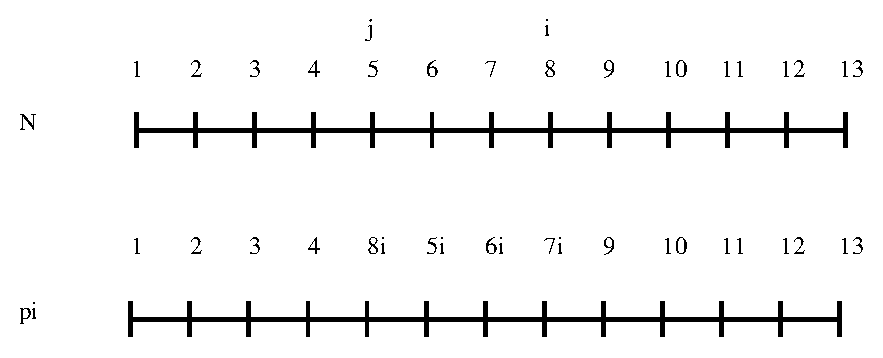
\includegraphics[scale=.5]{fig1.eps}
%%   \caption{Caso com $i = 8$ e $j = 5$.}
%%   \label{fig1}
%% \end{figure}

     
%Se $i < j$, então

Balas apresenta uma caracterização que determina o valor de $\pi(i)$ dentro de um intervalo de números inteiros. Para que haja também uma caracterização determinando o valor de $\pi^{-1}(i)$ (ou seja, os candidatos para a posição $i$) dentro de um intervalo de números inteiros, os valores $k(i)$ precisam atender ao seguinte: $k(i) - k(i+1) \leq 1$ para $i = 1, \dots, n$. Em geral, o que temos é a seguinte condição necessária mas não suficiente. Para qualquer solução viável do TSP restrito e generalizado, $j_{(i)} \leq \pi^{-1}(i) \leq j^{(i)}$ para qualquer posição $i$ desta solução sendo $$j_{(i)} := \min\{j: j + k(j) \geq i+1\},$$ $$j^{(i)} := \max\{j: j - i \leq |P_j|\}.$$ Como esta condição em geral é necessária mas não suficiente, para evitar criar vértices que não estarão em qualquer solução viável do problema, é também necessário verificar a condição do TSP restrito e generalizado: ao criar um vértice $(i, j, S^-_{ij}, S^+_{ij})$, devemos verificar para toda cidade $l$ ainda não visitada (em $S^+_{ij}$), a condição $\pi(l) < \pi(j)$, caso  $j \geq l + k(l)$. No trabalho de Balas e Simonetti \cite{BS}, os autores apresentam uma forma mais rápida para tratar este caso (veja sobre $kthresh(v)$ no próximo parágrafo). Para nosso intuito, vamos trabalhar com o teste mais lento (verificar todos os vértices em $S^+$), porém ainda polinomial no tamanho da entrada.

Um teste mais rápido para verificar se um vértice $v$ do grafo construído pertence a alguma solução inviável pode ser feita através de um limitante denotado $kthresh(v)$. Primeiro, é importante notar que um vértice $v=(i, j, S^-_{ij}, S^+_{ij})$ em uma solução viável do problema, implica que $k(j)$ é maior que a diferença entre a cidade de maior índice em $S^-$ e $j$ (pois, $l < j + k(j)$ para todo $l$ em $S^-_{ij}$ e assim, $k(j) > \max\{S^-_{ij}\} - j$). Para tratar $S^-_{ij} = \emptyset$, temos $k(j) > \max\{0, \max\{S^-_{ij}\}\} - j$. Dessa forma, $kthresh(v) = 1+\max\{0, \max\{S^-_{ij}\}\} - j$. Portanto, qualquer vértice $v=(i,j,S^-_{ij}, S^+_{ij})$ tal que $kthresh(v) > k(j)$ pertence a uma solução inviável e pode ser desconsiderado.

Para finalizar, agora vamos mostrar como Balas e Simonetti transformam o problema do TSP com janelas de tempos para o TSP restrito e generalizado. A ideia é usar as janelas para impor restrições de precedência: se $j \geq i + k(i)$, então $\pi(i) < \pi(j)$. Suponha que cada cidade $i$ tenha janelas de tempo definidas no intervalo $[a_i, b_i]$. Considere também $t_{ij}$, o tempo de viagem de $i$ até $j$. Em qualquer solução viável, uma cidade $i$ tem que preceder uma cidade $j$ se $a_j + t_{ji} > b_i$. Fixada uma cidade $i$, ao escolher a cidade $j_0$ com menor índice tal que $a_j + t_{ji} > b_i$ para toda cidade $j \geq j_0$, então podemos definir $k(i)=j_0 - i$. Para a cidade 1, $k(1) = 1$ e para as outras cidades, caso não exista tal $j_0$, então $j_0=n+1$.

\begin{figure}[ht]
  \centering
  \psfrag{k}{\small $k$}
  \psfrag{janela}{\small janela}
  \psfrag{j0-i}{\small $j_0-i$}
  \psfrag{5-2}{\small $5-2$}
  \psfrag{7-3}{\small $7-3$}
  \psfrag{5-4}{\small $5-4$}
  \psfrag{8-5}{\small $8-5$}
  \psfrag{8-6}{\small $8-6$}
  \psfrag{8-7}{\small $8-7$}
  \psfrag{1}{\small 1}
  \psfrag{2}{\small 2}
  \psfrag{3}{\small 3}
  \psfrag{4}{\small 4}
  \psfrag{5}{\small 5}
  \psfrag{6}{\small 6}
  \psfrag{7}{\small 7}
  \psfrag{8}{\small 8}
  \psfrag{9}{\small 9}
  \psfrag{i}{\small $i$}
  \psfrag{N}{$N$}
  \psfrag{pi}{$\pi$}
  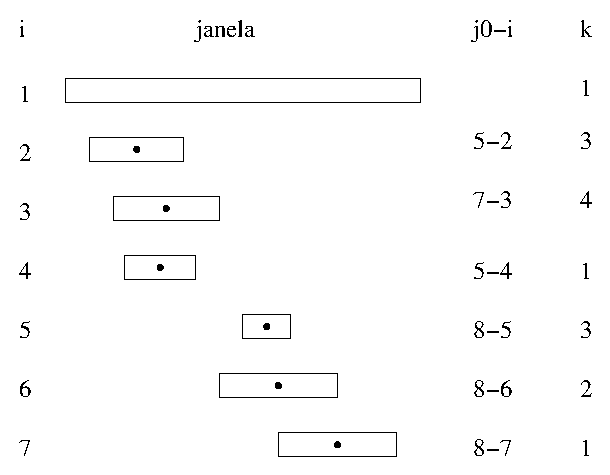
\includegraphics[scale=.7]{fig2.eps}
  \caption{Caso com $t_{ji} = 0$. Mesmo exemplo presente no trabalho de Balas e Simonetti.}
  \label{fig2}
\end{figure}

Alterar a ordem das cidades pode alterar os $k(i)$'s encontrados. Quanto menor for $k= \max_{i=1, \dots, n}\{k(i)\}$, melhor será o desempenho do algoritmo, já que o tempo de execução depende exponenciamente de tal $k$. Balas e Simonetti comentam que encontrar tal $k$ talvez seja NP-difícil \cite{BS}.

\section*{TSP com carro elétrico - \textit {Electric Travaling Salasmen Problem with Time Windows} (E-TSPTW)}
A partir daqui, vamos também usar a notação presente no artigo de Roberti e Wen \cite{RW}.

O conjunto de vértices é $V = \{o, d\} \cup C \cup S$, onde $o$ é a origem $d$ é o destino (uma cópia da origem), $C$ é o conjunto de $n$ clientes a visitar e $S$ é o conjunto de $m$ estações de recarga. Uma janela de tempo $[e_i, l_i]$ é defida para a origem, destino, e elemento $i$ de $C$. Tanto $e_i$ quanto $l_i$ são números inteiros positivos. As janelas de tempo são \emph{duras} ({\it hard}), ou seja, um vértice $i$ pode ser visitado antes de $e_i$ mas não depois de $l_i$. As estações de recarga estão sempre disponíveis. Entre os vértices $i$ e $j$ de $V$ temos a distância entre eles ($d_{ij}$), o tempo entre eles ($t_{ij}$) e o consumo de bateria ao percorrer $d_{ij}$ ($q_{ij}$). Todos números inteiros positivos. O consumo de bateria é dado por $q_{ij} = hd_{ij}$, sendo $h$ a taxa de consumo igual para todos os arcos do grafo de entrada. O tempo de recarga é linear em relação à quantidade a ser carregada (taxa de recarga é igual a $g$ e vale para todas as estações). Em uma solução viável, uma recarga pode ser realizada muitas vezes em uma única estação. O vértice origem é também uma estação de recarga. No presente trabalho de iniciação científica, consideramos a recarga total da bateria. Mas existem trabalhos que consideram recarga parcial. Uma solução viável começa na origem, termina no destino e passa por todos os clientes uma única vez, dentro da correspondente janela de tempo, podendo passar por estações de recarga. Em nenhum momento, a bateria pode acabar. A solução ótima é uma viável com a menor distância percorrida possível. Consideramos $d_{ij} = t_{ij}$ para todo arco $(i,j)$.

É importante destacar a seguinte propriedade do algoritmo de programação dinâmica de Balas. Dada que uma cidade foi visitada na posição $i$, o algoritmo considera todas as possíveis cidades que poderíam ocupar a posição $i+1$, ou seja, as cidade candidatas de $\pi^{-1}(i+1)$. No algoritmo de Balas, o caixeiro viajante sai de uma cidade $u$ visitada na posição $i$ e vai direto para a próxima cidade $v$ na posição $i+1$. A adaptação do algoritmo de Balas para o E-TSPTW considera que o caixeiro ou vai direto de $u$ para $v$; ou passa para recarregar a bateria em alguma estação de recarga. Lembre que denotamos por $(i,j,S^-_{ij},S^+_{ij})$ um vértice do grafo auxiliar que visita a cidade $j$ na posição $i$ com os conjuntos $S^-$ e $S^+$ definidos em função da compatibilidade entre vértices do grafo. Para o caso do E-TSPTW, vamos denotar por $(i, j, S^-_{ij}, S^+_{ij}, q, c)$, sendo $q$ a bateria do carro elétrico no vértice e $c$ um custo neste vértice que corresponde a um caminho que começa na origem, termina em $j$ e passa pelas cidades em $\{N_{i} \backslash S^+_{ij}\} \cup S^-_{ij}$. Outra forma de denotar a bateria e o custo em um vértice $v$ do grafo auxiliar é por $q(v)$ e $c(v)$, respectivamente. É importante notar que caminhos que iniciam na cidade 1, terminam na cidade $w$ podem ter diferentes cargas de bateria e diferentes custos. Como neste caso estamos tratando a recarga de bateria, precisamos manter vértices que se poderiam se diferenciar somente na carga da bateria que o carro terá e no custo. O mapa da Figura \ref{fig3} ilustra um exemplo. Observe na figura que temos o caminho $u \rightarrow v \rightarrow x \rightarrow w$ e o caminho $u  \rightarrow x  \rightarrow v  \rightarrow w$. No grafo auxiliar construído pelo algoritmo de Balas e adaptado para tratar o carro elétrico, teremos possivelmente dois vértices para representar estes dois caminhos. Os vértices são $v=(i, w, (S^-_{iw}), (S^+_{iw}), q, c)$ e $v^{\prime}=(i, w, (S^-_{iw})^{\prime}, (S^+_{iw})^\prime, q^\prime, c^\prime)$. Eventualmente, podemos remover um desses vértices do grafo auxiliar, caso $S^-_{iw} = (S^-_{iw})^\prime$ e $S^+_{iw} = (S^+_{iw})^\prime$, então podemos eventualmente remover o vértice do grafo auxiliar correspondente ao caminho 1 (2), se $q(v) \leq q(v^\prime)$ e $c(v) \geq c(v^\prime)$ ($q(v^\prime) \leq q(v)$ e $c(v^\prime) \geq c(v)$), ou seja, caso foram percorridas as mesmas cidades em caminhos entre 1 e $w$, a bateria no vértice $v$ é menor e o custo no vértice $v$ é maior. Então, podemos eliminar o vértice $v$. Caso contrário (ou exclusivo), precisamos manter ambos os vértices no grafo auxiliar. 

\begin{figure}[ht]
  \centering
  \psfrag{k}{\small $k$}
  \psfrag{janela}{\small janela}
  \psfrag{j0-i}{\small $j_0-i$}
  \psfrag{5-2}{\small $5-2$}
  \psfrag{7-3}{\small $7-3$}
  \psfrag{5-4}{\small $5-4$}
  \psfrag{8-5}{\small $8-5$}
  \psfrag{8-6}{\small $8-6$}
  \psfrag{8-7}{\small $8-7$}
  \psfrag{1}{\small 1}
  \psfrag{2}{\small 2}
  \psfrag{w}{\small $w$}
  \psfrag{v}{\small $v$}
  \psfrag{u}{\small $u$}
  \psfrag{x}{\small $x$}
  \psfrag{7}{\small 7}
  \psfrag{8}{\small 8}
  \psfrag{9}{\small 9}
  \psfrag{i}{\small $i$}
  \psfrag{N}{$N$}
  \psfrag{pi}{$\pi$}
  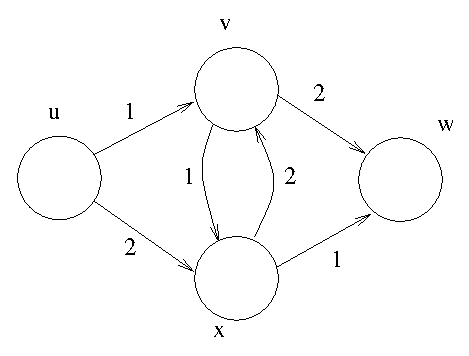
\includegraphics[scale=.7]{fig3.eps}
  \caption{Dois caminhos de $u$ para $w$ com custo e consumo de bateria diferentes.}
  \label{fig3}
\end{figure}

\medskip
\printbibliography

\end{document}
